\chapter{Implementacija i korisničko sučelje}
		
		
		\section{Korištene tehnologije i alati}
		
			
			\noindent Komunikacija u timu je ostvarena putem aplikacija \underline{WhatsApp}\footnote{https://www.whatsapp.com/} i \underline{Microsoft Teams}\footnote{https://www.microsoft.com/hr-hr/microsoft-365/microsoft-teams/group-chat-software}. Aplikacija WhatsApp korištena je isključivo za slikovno-tekstualnu komunikaciju, dok je Microsoft Teams korišten za telekonferencijski kontakt. Kao sustav za upravljanje izvornim kodom korišten je \underline{Git}\footnote{https://git-scm.com/}, dok se udaljeni repozitorij projekta nalazi na web platformi \underline{Git Lab}\footnote{https://about.gitlab.com/}. Za izradu UML dijagrama korišten je \underline{Astah UML}\footnote{https://astah.net/}.
			
			\noindent Od alata za razvojno okruženje korišteni su \underline{PyCharm}\footnote{https://www.jetbrains.com/pycharm/} i \underline{Notepad++}\footnote{https://notepad-plus-plus.org/downloads/}. PyCharm je razvojno sučelje koje se koristi za programiranje u Pythonu. Od velike je pomoći kod pisanja koda s laganom navigacijom unutar programa. Notepad++ je dobar za uređenje teksta i izvornog koda za upotrebu u sustavu Microsoft Windows.
			
			\noindent Korištena baza podataka je \underline{PostgreSQL}\footnote{https://www.postgresql.org/}, a nalazi se na poslužitelju u oblaku \underline{Heroku}\footnote{https://www.heroku.com/}.
			
			\noindent Za izradu backenda korišteni su \underline{Python}\footnote{https://www.python.org/} i \underline{Django}\footnote{https://www.djangoproject.com/}, a za frontend \underline{Bootstrap}\footnote{https://getbootstrap.com/}.
			
			\noindent Python (Guido van Rossum, 1990.) programski je jezik opće namjene koji dopušta nekoliko stilova programiranja (objektno orijentirano, strukturno i aspektno orijentirano programiranje).
			
			\noindent Django je besplatan i open-source web framework koji se temelji na Pythonu. Olakšava stvaranje složenih web stanica.
			
			\noindent Bootstrap je frontend framework i besplatna open-source kolekcija HTML CSS i java script alata za kreiranje web stranica i web aplikacija.
			
			\noindent Za pisanje dokumentacije korišten je alat TeXstudio.
			
			
			
			\eject 
		
	
		\section{Ispitivanje programskog rješenja}
	
			
			\subsection{Ispitivanje komponenti}
			
		U nastavku se nalazi 6 unit testova (izvorni kod i rezultat ispitivanja) numeriranih od 1 do 6.
		
		\begin{figure}[H]
			\centerfloat
			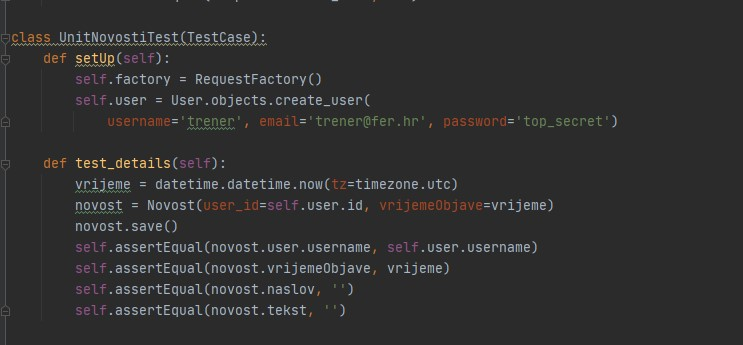
\includegraphics[scale=0.55]{slike/unittest1izv.jpeg} %veličina slike u odnosu na originalnu datoteku i pozicija slike
			\caption{Izvorni kod unit testa 1}
			
		\end{figure}
	
	\begin{figure}[H]
		\centerfloat
		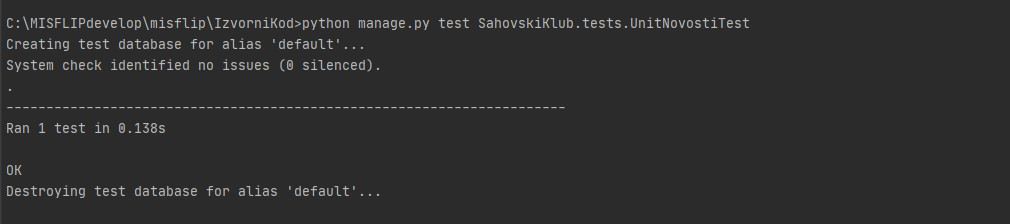
\includegraphics[scale=0.55]{slike/unittest1.jpeg} %veličina slike u odnosu na originalnu datoteku i pozicija slike
		\caption{Rezultat ispitivanja unit testa 1}
		
	\end{figure}

\begin{figure}[H]
	\centerfloat
	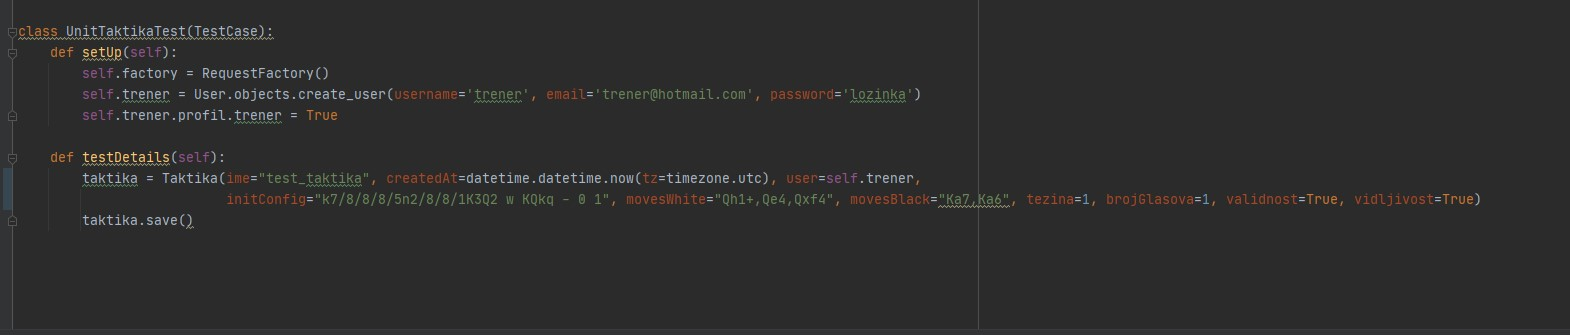
\includegraphics[scale=0.40]{slike/unittest2izv.jpeg} %veličina slike u odnosu na originalnu datoteku i pozicija slike
	\caption{Izvorni kod unit testa 2}
	
\end{figure}
	
	\begin{figure}[H]
		\centerfloat
		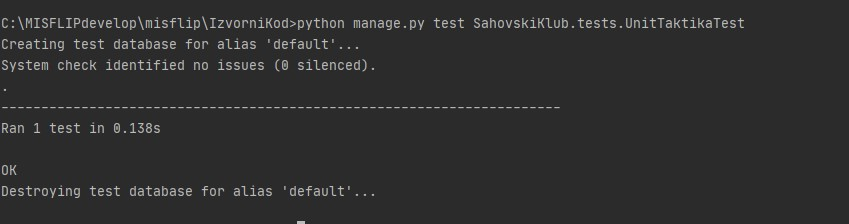
\includegraphics[scale=0.55]{slike/unittest2.jpeg} %veličina slike u odnosu na originalnu datoteku i pozicija slike
		\caption{Rezultat ispitivanja unit testa 2}
		
	\end{figure}

\begin{figure}[H]
	\centerfloat
	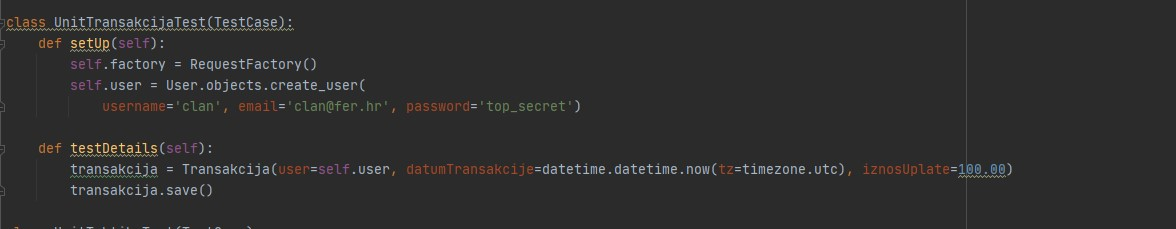
\includegraphics[scale=0.55]{slike/unittest3izv.jpeg} %veličina slike u odnosu na originalnu datoteku i pozicija slike
	\caption{Izvorni kod unit testa 3}
	
\end{figure}

\begin{figure}[H]
	\centerfloat
	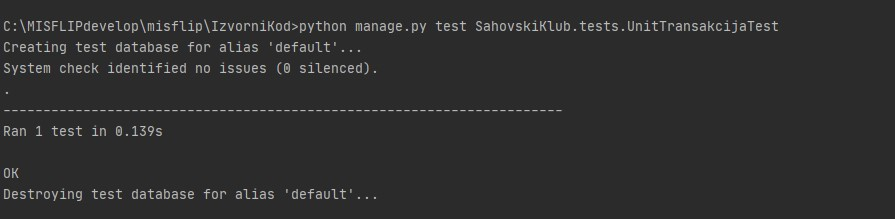
\includegraphics[scale=0.55]{slike/unittest3.jpeg} %veličina slike u odnosu na originalnu datoteku i pozicija slike
	\caption{Rezultat ispitivanja unit testa 3}
	
\end{figure}

\begin{figure}[H]
	\centerfloat
	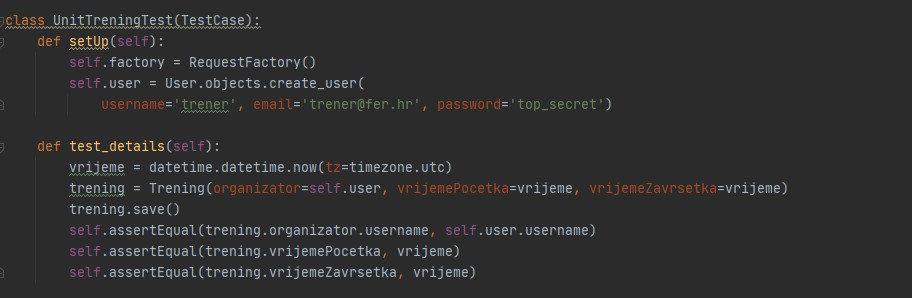
\includegraphics[scale=0.55]{slike/unittest4izv.jpeg} %veličina slike u odnosu na originalnu datoteku i pozicija slike
	\caption{Izvorni kod unit testa 4}
	
\end{figure}

\begin{figure}[H]
	\centerfloat
	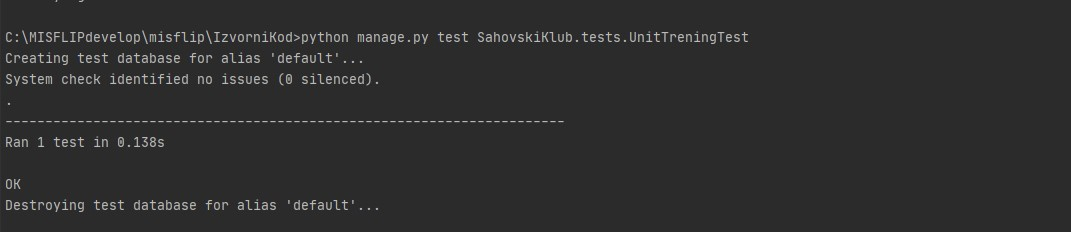
\includegraphics[scale=0.55]{slike/unittest4.jpeg} %veličina slike u odnosu na originalnu datoteku i pozicija slike
	\caption{Rezultat ispitivanja unit testa 4}
	
\end{figure}

\begin{figure}[H]
	\centerfloat
	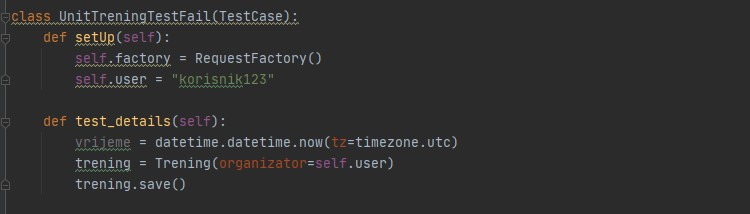
\includegraphics[scale=0.55]{slike/unittest5izv.jpeg} %veličina slike u odnosu na originalnu datoteku i pozicija slike
	\caption{Izvorni kod unit testa 5}
	
\end{figure}

\begin{figure}[H]
	\centerfloat
	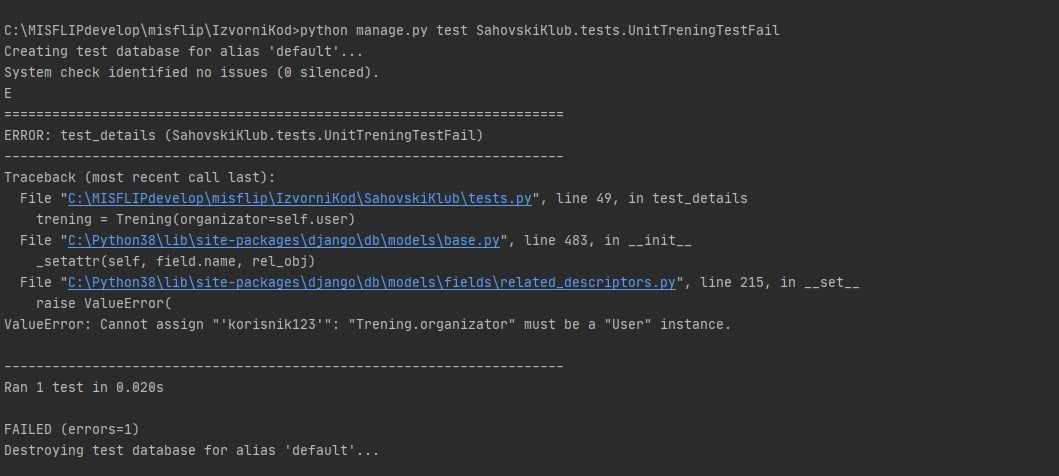
\includegraphics[scale=0.55]{slike/unittest5.jpeg} %veličina slike u odnosu na originalnu datoteku i pozicija slike
	\caption{Rezultat ispitivanja unit testa 5}
	
\end{figure}

\begin{figure}[H]
	\centerfloat
	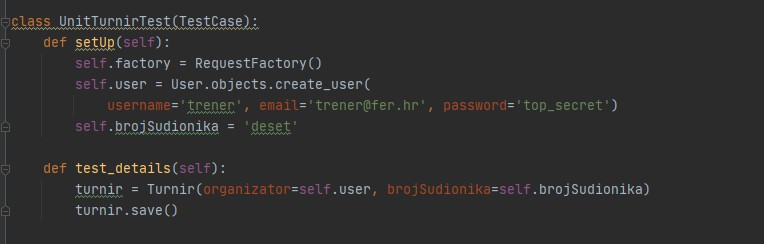
\includegraphics[scale=0.55]{slike/unittest6izv.jpeg} %veličina slike u odnosu na originalnu datoteku i pozicija slike
	\caption{Izvorni kod unit testa 6}
	
\end{figure}

\begin{figure}[H]
	\centerfloat
	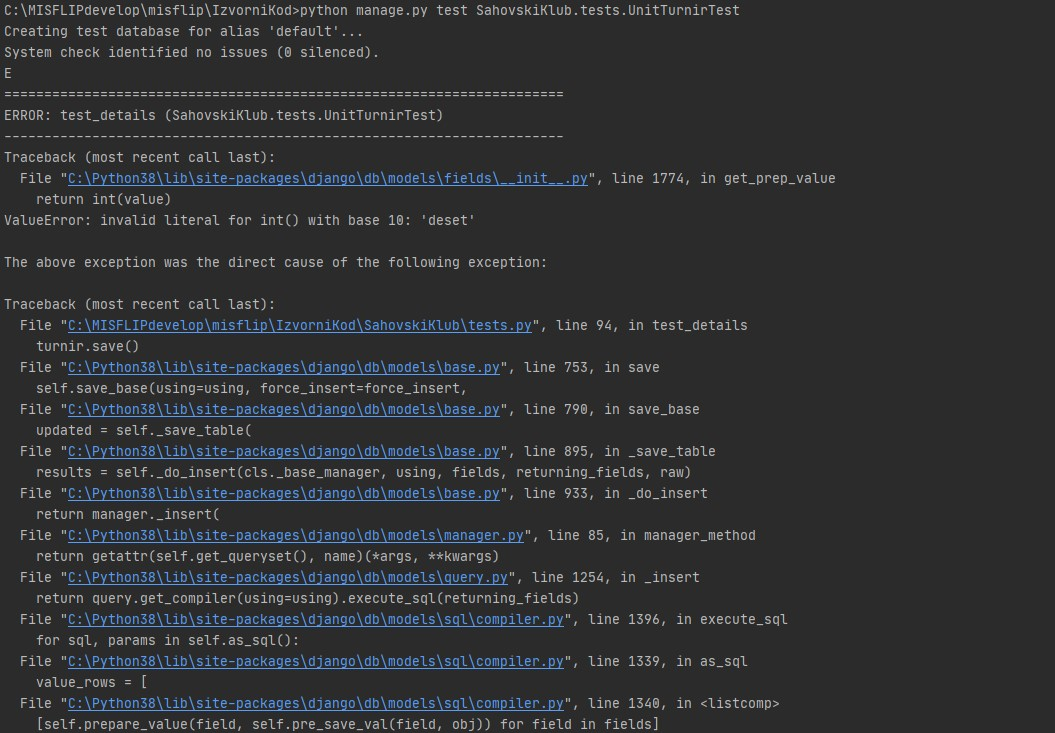
\includegraphics[scale=0.55]{slike/unittest6-1.jpeg} %veličina slike u odnosu na originalnu datoteku i pozicija slike
	\caption{Rezultat ispitivanja unit testa 6 - 1. dio}
	
\end{figure}

\begin{figure}[H]
	\centerfloat
	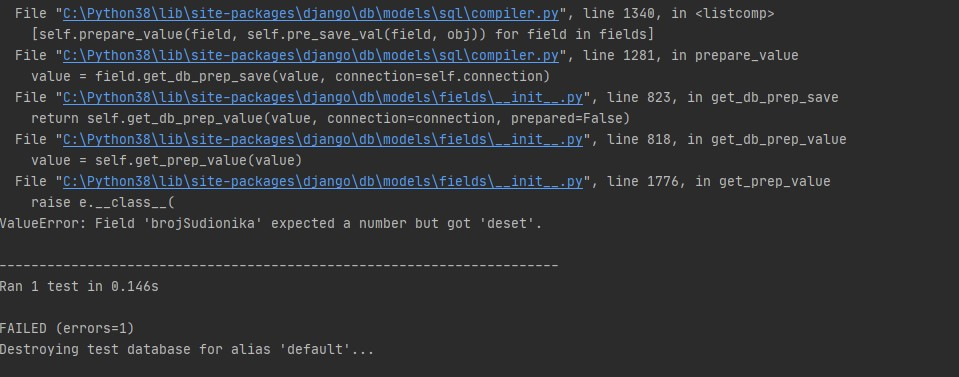
\includegraphics[scale=0.55]{slike/unittest6-2.jpeg} %veličina slike u odnosu na originalnu datoteku i pozicija slike
	\caption{Rezultat ispitivanja unit testa 6 - 2. dio}
\end{figure}
		
			
			\subsection{Ispitivanje sustava}
			
			U nastavku se nalaze 4 slučajeva ispitivanja sustava (izvorni kod i rezultat ispitivanja) numeriranih od 1 do 4.
			
			 	\begin{figure}[H]
			 	\centerfloat
			 	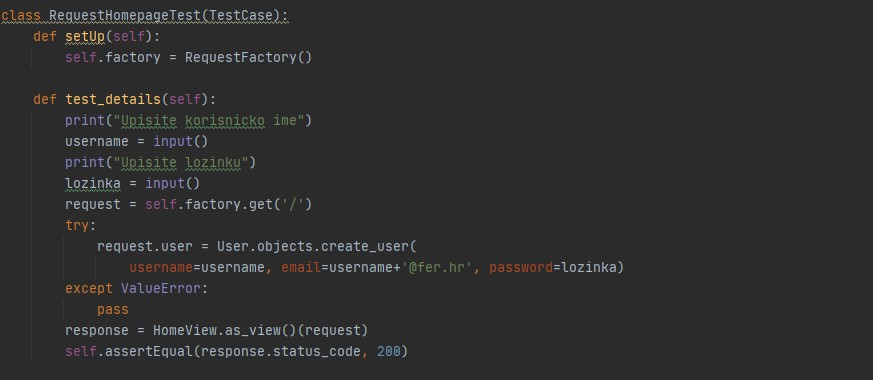
\includegraphics[scale=0.55]{slike/ispitivanjesustava1izv.jpeg} %veličina slike u odnosu na originalnu datoteku i pozicija slike
			 	\caption{Izvorni kod ispitivanja sustava 1}
			 	
			 \end{figure}
			 
			 \begin{figure}[H]
			 	\centerfloat
			 	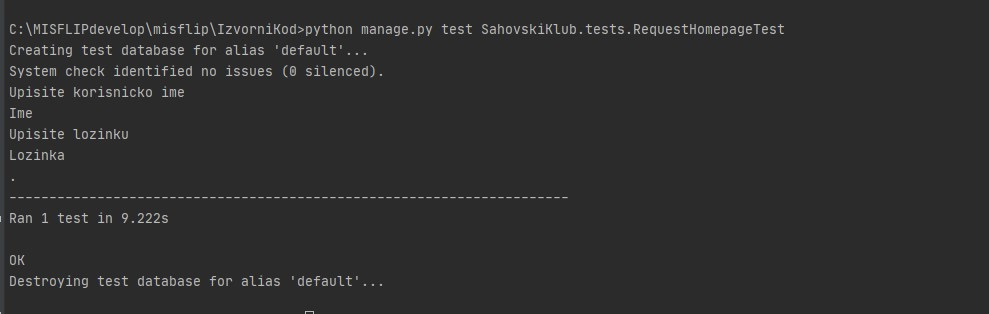
\includegraphics[scale=0.55]{slike/ispitivanjesustava1.jpeg} %veličina slike u odnosu na originalnu datoteku i pozicija slike
			 	\caption{Rezultat ispitivanja sustava 1}
			 	
			 \end{figure}
			 
			 \begin{figure}[H]
			 	\centerfloat
			 	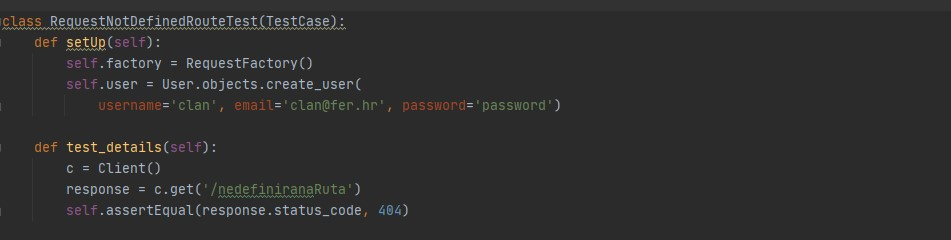
\includegraphics[scale=0.55]{slike/ispitivanjesustava2izv.jpeg} %veličina slike u odnosu na originalnu datoteku i pozicija slike
			 	\caption{Izvorni kod ispitivanja sustava 2}
			 	
			 \end{figure}
			 
			 \begin{figure}[H]
			 	\centerfloat
			 	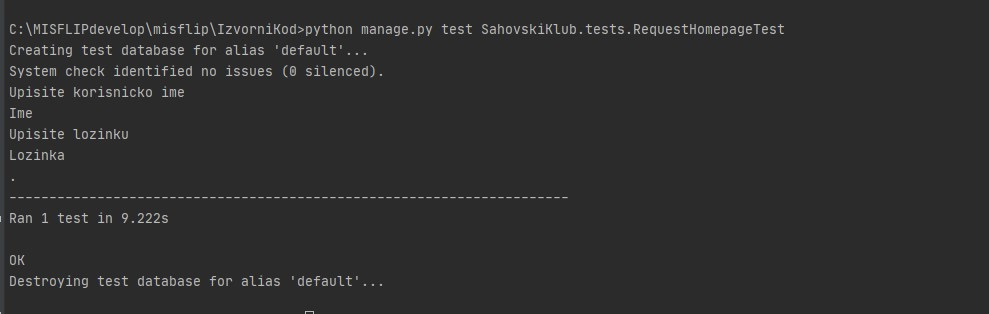
\includegraphics[scale=0.55]{slike/ispitivanjesustava1.jpeg} %veličina slike u odnosu na originalnu datoteku i pozicija slike
			 	\caption{Rezultat ispitivanja sustava 2}
			 	
			 \end{figure}
			 
			 \begin{figure}[H]
			 	\centerfloat
			 	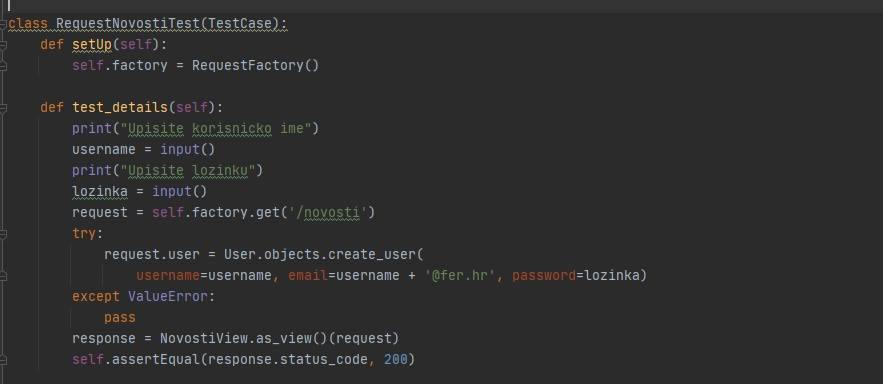
\includegraphics[scale=0.55]{slike/ispitivanjesustava3izv.jpeg} %veličina slike u odnosu na originalnu datoteku i pozicija slike
			 	\caption{Izvorni kod ispitivanja sustava 3}
			 	
			 \end{figure}
			 
			 \begin{figure}[H]
			 	\centerfloat
			 	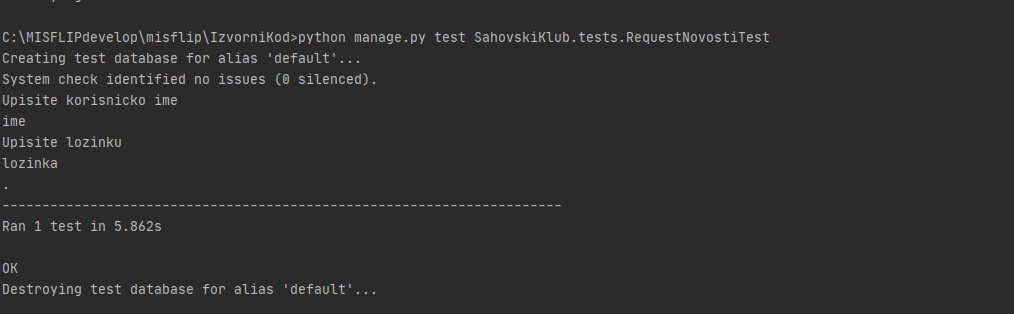
\includegraphics[scale=0.55]{slike/ispitivanjesustava3.jpeg} %veličina slike u odnosu na originalnu datoteku i pozicija slike
			 	\caption{Rezultat ispitivanja sustava 3}
			 	
			 \end{figure}
			 
			 \begin{figure}[H]
			 	\centerfloat
			 	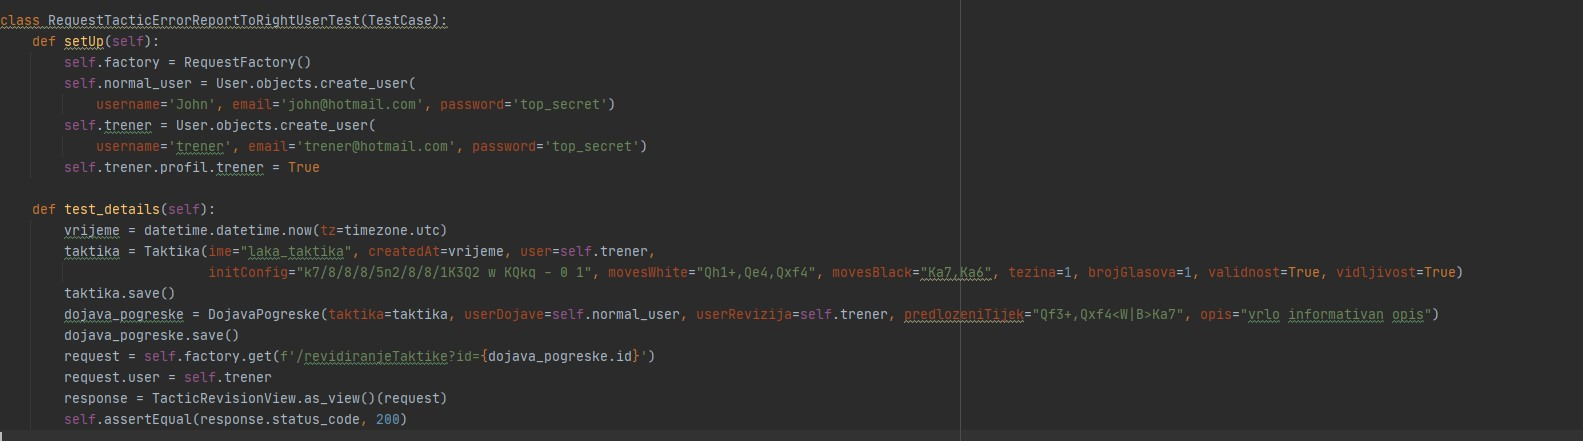
\includegraphics[scale=0.40]{slike/ispitivanjesustava4izv.jpeg} %veličina slike u odnosu na originalnu datoteku i pozicija slike
			 	\caption{Izvorni kod ispitivanja sustava 4}
			 	
			 \end{figure}
			 
			 \begin{figure}[H]
			 	\centerfloat
			 	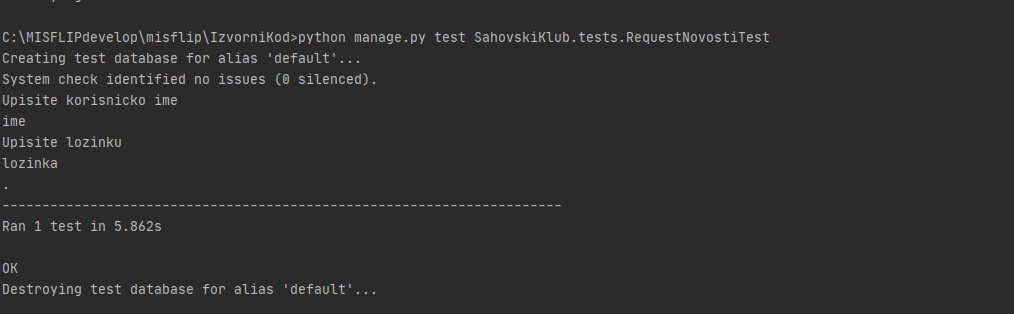
\includegraphics[scale=0.55]{slike/ispitivanjesustava3.jpeg} %veličina slike u odnosu na originalnu datoteku i pozicija slike
			 	\caption{Rezultat ispitivanja sustava 4}
			 	
			 \end{figure}
			
			\eject 
		
		
		\section{Dijagram razmještaja}
			
			
			Na slici 5.22 prikazan je dijagram razmještaja. Na poslužiteljskom računalu se nalaze web poslužitelj i poslužitelj baze padataka MISFLIP. Za pristup web aplikaciji Šahovski klub, klijent se služi web preglednikom. Sustav je baziran na arhitekturi klijent-poslužitelj. Komunikacija između korisnikovog računala (neregistrirani korisnik, član, trener, administrator) i poslužitelja odvija se preko HTTPS veze.
			
			\begin{figure}[H]
				\centerfloat
				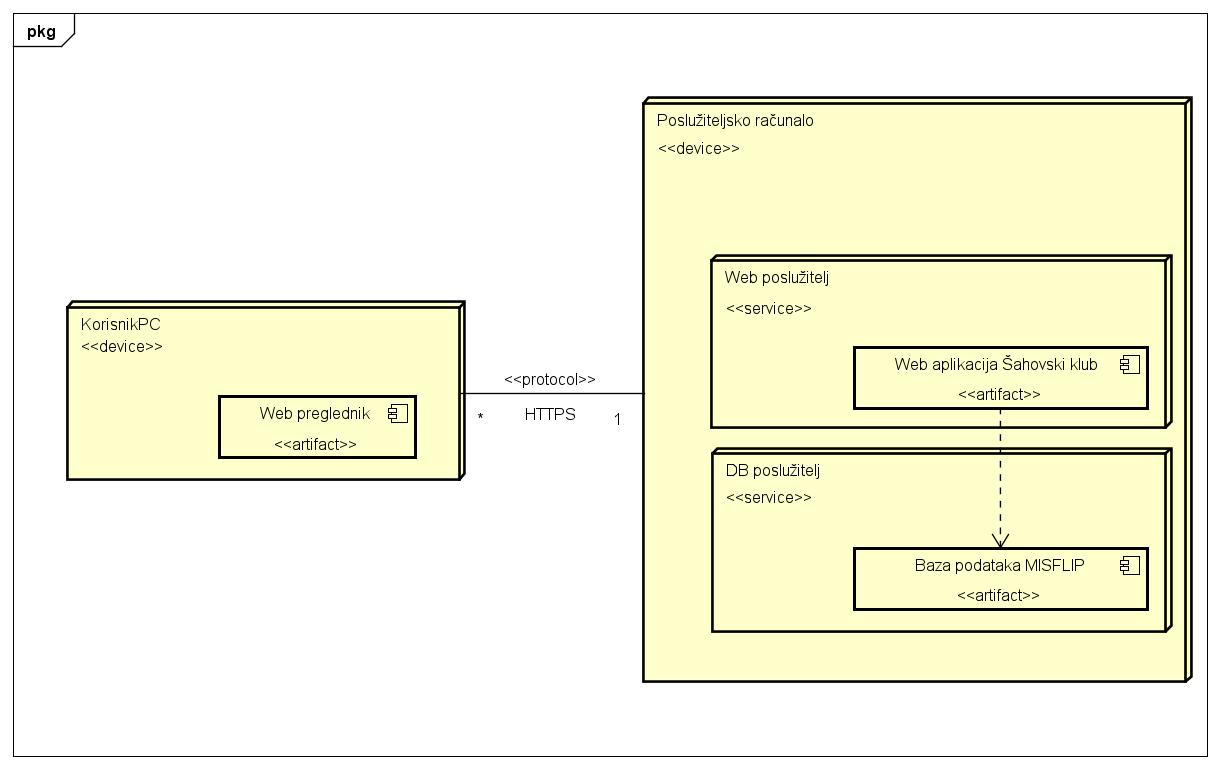
\includegraphics[scale=0.40]{dijagrami/Dijagramrazmjestaja.jpg} %veličina slike u odnosu na originalnu datoteku i pozicija slike
				\caption{Dijagram razmještaja}
				
			\end{figure}
			
			\eject
		
		\section{Upute za puštanje u pogon}
		
			\noindent Za početak potrebno je otići na stranicu \url{https://www.heroku.com/} i registrirati se. 
			
			\noindent U sljedećem koraku treba otvoriti Command Prompt i pozicionirati se u mapu IzvorniKod unutar projekta.
			
			\noindent Treba upisati naredbu "heroku login" i potom pritisnuti bilo koji gumb izuzevši q pri čemu se otvara stranica na web pregledniku gdje je potrebno prijaviti se s podacima koji su kreirani putem registracije.
			
			\noindent Potom se u Command Promptu upisuje naredba „heroku create“ pri čijem izvršavanju se dobije ime servera.
			
			\begin{figure}[H]
				\centerfloat
				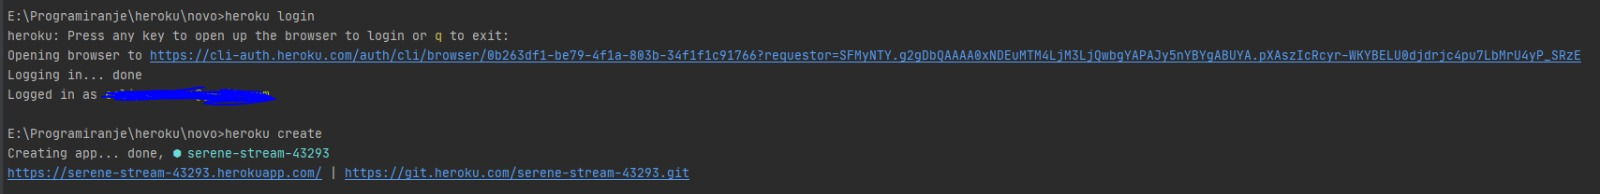
\includegraphics[scale=0.3]{slike/pustanjeupogon1.jpeg} %veličina slike u odnosu na originalnu datoteku i pozicija slike
				\caption{Podešavanje u Command Promptu 1}
				
			\end{figure}
			
			\noindent Sljedeće treba upisat "git init", a nakon toga "heroku git:remote -a“, i uz ovu naredbu se navodi ime heroku servera koji je dobiven u prethodnom koraku npr. „serene-stream-43293“.
			
			\noindent Nakon toga u datoteku settings.py u ALLOWED\texttt{\char`_}HOSTS treba staviti ime heroku servera i završiti sa ''.herokuapp.com'' npr. ''serene-stream-43293.herokuapp.com''. 
			
			\noindent Nakon što je to napravljeno u Command Promptu upisuje se naredba "git add .“.
			
			\begin{figure}[H]
				\centerfloat
				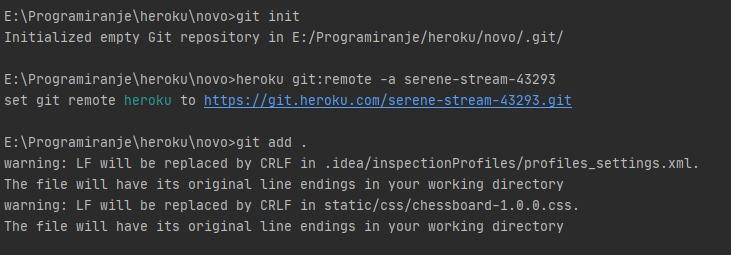
\includegraphics[scale=0.4]{slike/pustanjeupogon2.jpeg} %veličina slike u odnosu na originalnu datoteku i pozicija slike
				\caption{Podešavanje u Command Promptu 2}
				
			\end{figure}
			
			\eject
			
			\noindent Zatim se upisuje "git commit -m "message"" (pri čemu message može biti bilo koji niz znakova npr. "initial commit").
			
			\begin{figure}[H]
				\centerfloat
				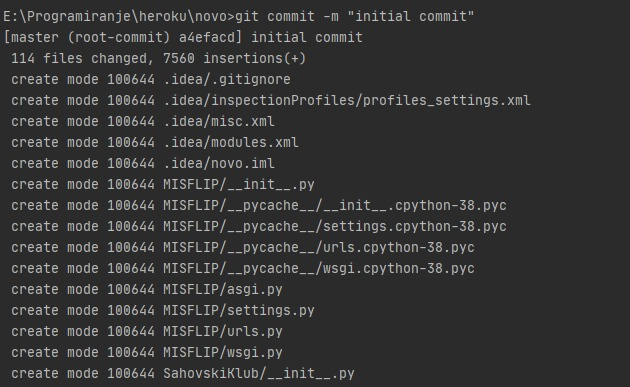
\includegraphics[scale=0.4]{slike/pustanjeupogon3.jpeg} %veličina slike u odnosu na originalnu datoteku i pozicija slike
				\caption{Podešavanje u Command Promptu 3}
				
			\end{figure}
			
			\noindent Na kraju se upisuje "git push heroku master“, te je time aplikacija namještena.
			
			\begin{figure}[H]
				\centerfloat
				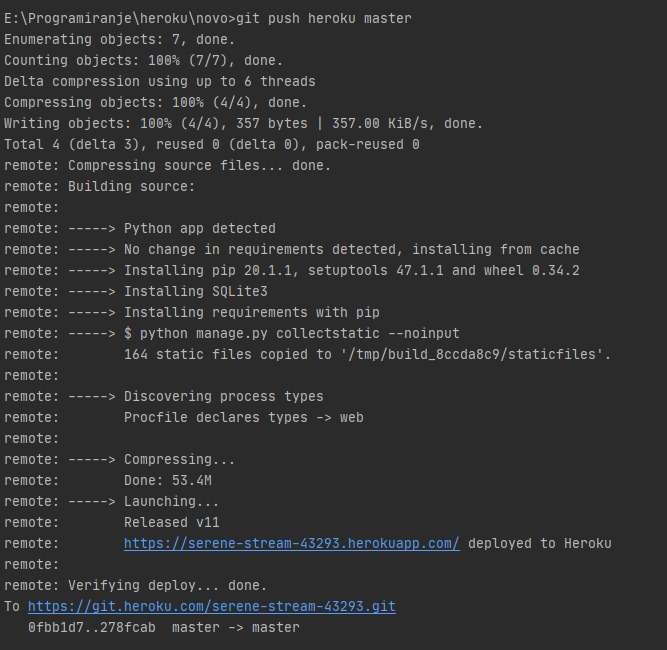
\includegraphics[scale=0.4]{slike/pustanjeupogon4.jpeg} %veličina slike u odnosu na originalnu datoteku i pozicija slike
				\caption{Podešavanje u Command Promptu 4}
				
			\end{figure}
			
			\eject 